\documentclass{article}


\usepackage{PRIMEarxiv}

\usepackage[utf8]{inputenc} % allow utf-8 input
\usepackage[T1]{fontenc}    % use 8-bit T1 fonts
\usepackage{hyperref}       % hyperlinks
\usepackage{url}            % simple URL typesetting
\usepackage{booktabs}       % professional-quality tables
\usepackage{amsfonts}       % blackboard math symbols
\usepackage{nicefrac}       % compact symbols for 1/2, etc.
\usepackage{microtype}      % microtypography
\usepackage{lipsum}
\usepackage{graphicx}
\usepackage{enumitem}
% \graphicspath{{media/}}     % organize your images and other figures under media/ folder

  
%% Title
\title{Centralized PPO in Multi-Agent Reinforcement Learning
%%%% Cite as
%%%% Update your official citation here when published 
\thanks{\textit{\underline{Citation}}: 
\textbf{Authors. Title. Pages.... DOI:000000/11111.}} 
}

\author{
  Anish Sahoo \\
  CS 4180 \\
  Northeastern University \\
  Boston, MA\\
  \texttt{sahoo.an@northeastern.edu} \\
}


\begin{document}
\maketitle


\begin{abstract}
This paper explores the use of centralized Proximal Policy Optimization (PPO) in multi-agent 
reinforcement learning. We use the KnightsArchersZombies environment from PettingZoo to train 
a model for multiple agents with a centralized, shared actor-critic model. We implement a version of PPO inspired
by the original PPO paper and the MAPPO paper. We observe that the centralized PPO model without
any temporal data converges to a suboptimal policy. We then update our model to include temporal data
and observe that the model converges to a much better policy. We also observe some emergent behavior
that suggests that the agents are learning to cooperate. We conclude that centralized PPO with temporal
data is a promising approach to multi-agent reinforcement learning that encourages cooperation 
and generalization.

\end{abstract}


% keywords can be removed
% \keywords{PPO \and PettingZoo \and On Policy \and Multi-Agent \and Reinforcement Learning}


\section{Introduction}
Multi-agent reinforcement learning (MARL) is a branch of reinforcement learning that focuses on
training multiple agents to interact with each other and their environment. MARL is a challenging
problem because the agents must learn to cooperate and compete with each other in a complex,
dynamic environment. The KnightsArchersZombies environment presents a unique challenge, simulating 
a scenario where different agent types (knights, archers, and zombies) interact 
within a 720 by 1280 pixel map. Each agent type possesses unique characteristics 
and capabilities, creating complex interaction dynamics that make it hard to learn optimal policies.

This research focuses on Proximal Policy Optimization (PPO), a 
state-of-the-art policy gradient method. Introduced by OpenAI \cite{DBLP:journals/corr/SchulmanWDRK17} in 2017, 
PPO has become very popular in the reinforcement learning community 
due to its ability to balance exploration and 
exploitation while being very sample efficient. Additionally, due to its clipped objective,
PPO is known for being more stable than other policy gradient methods like REINFORCE.

We implement a specific configuration of PPO that aims to be more efficient and effective in
multi-agent environments. Instead of using separate actor-critic models for each agent 
like in the MAPPO paper \cite{DBLP:journals/corr/abs-2103-01955}, we implement a
centralized, shared actor-critic model that allows agents to share information
and perhaps learn from each other. By leveraging this version of PPO, we aim to investigate if agents can 
learn from each other and develop effective strategies. We hypothesize that this 
centralized model will enable agents to develop more effective strategies by 
leveraging the collective knowledge of the group.

Our study seeks to understand how this version of PPO performs in this environment and
whether the centralized shared model can help agents learn effective strategies.

\section{Methodology}
\label{sec:headings}

\subsection{Environment}
Knights Archers Zombies is a multi-agent environment from PettingZoo butterfly family of environments.
The environment consists of three types of agents: knights, archers, and zombies. The knights and archers
are controlled by agent(s), while the zombies are controlled by the environment. The goal of the knights
and archers is to kill the zombies, while the goal of the zombies is to kill the knights and archers. 
Zombies are spawned randomly on the top of the 720 by 1280 pixel map, while knights and archers are spawned
on the bottom of the map. The agents die when they collide with a zombie. 

The environment can be formally defined as a Markov Decision Process (MDP) for each agent:
\begin{itemize}
  \item $\mathcal{S} = \{ s \in [0, 255]^{512 \times 512 \times 3} \}$, where each state is a 512 by 512 pixel RGB image of the area around the agent
  \item $\mathcal{A} = \{$ UP, DOWN, LEFT, RIGHT, ATTACK $\}$
  \item $\mathcal{R}(s, a)$: $+1$ for killing a zombie, otherwise $0$
  \item $\mathcal{T}(s'|s,a)$: The environment is deterministic in agent movement but stochastic in zombie movement/spawning.
\end{itemize}

An episode ends in one of the following scenarios:
\begin{itemize}
  \item All knights and archers are dead
  \item All zombies are dead
  \item A zombie reaches the bottom of the map
\end{itemize}

We will evaluate whether the agents can learn to play by observing the total reward accumulated over an episode. If the policy is very good, 
the agents should be able to kill most the zombies without any of the knights or archers dying. A good baseline reward would be around 25-30 per episode.

\subsection{The PPO Algorithm}
\label{sec:subheadings}
Proximal Policy Optimization (PPO) is a policy gradient method that aims to maximize the expected return
of an agent by updating its policy in the direction that increases the return. PPO is an on-policy method,
meaning that it learns from fresh data it has collected using the current policy. This makes PPO more sample efficient
than off-policy methods like DDPG and DQN. 

PPO is supported by two key ideas: the clipped objective and the importance ratio. The equation for the clipped objective is:
\begin{equation}
  L(\theta) = \mathbb{E} \left[ \min \left( r_t(\theta) \hat{A}_t, clip(r_t(\theta), 1 - \epsilon, 1 + \epsilon) \hat{A}_t \right) \right]
\end{equation}
In this equation, $\displaystyle r_t(\theta) = \frac{\pi_{\theta}(a_t|s_t)}{\pi_{\theta_{old}}(a_t|s_t)}$ is the importance ratio.

The clipped objective
is a modification to the policy gradient objective that prevents the policy from changing too much in one
direction. This helps stabilize the learning process and prevent the policy from diverging.

The importance ratio
is the ratio of the probability of taking an action under the new policy to the probability of taking the same
action under the old policy. This ratio is used to adjust the policy update in the direction that increases the return.

The PPO algorithm can be summarized as follows:
\begin{enumerate}
  \item Collect data by running the current policy in the environment
  \item Compute the advantage function using the collected data
  \item Compute the policy gradient using the advantage function
  \item Update the policy using the policy gradient
  \item Repeat until convergence
\end{enumerate}

PPO usually involves training a neural network to approximate the policy and value function. The policy
network takes the state as input and outputs the probability distribution over actions, while the value network
takes the state as input and outputs the value of the state. The policy network is updated using the policy gradient,
while the value network is updated using the value loss.

\pagebreak

We implement a 'centralized' version which has the following key differences:
\begin{enumerate}
  \item Shared actor-critic model - The Actor and Critic networks share the same weights
  \item Centralized training and decisions - All agents use the same network to learn and make decisions
  \item Centralized data collection - All agents share the same data buffer
\end{enumerate}

As this is a multi-agent problem, we also incorporate some features from the MAPPO\cite{DBLP:journals/corr/abs-2103-01955} paper to improve the performance of the model:
\begin{enumerate}
  \item GAE - We use the Generalized Advantage Estimation (GAE) to compute the advantage function
  \item Entropy regularization - We use entropy regularization to encourage exploration
  \item Temporal Data - In our second implementation, we incorporate temporal data by stacking frames
\end{enumerate}

% \section{Implementation and Results}

\section{Initial Implementation: No Temporal Data}

\subsection{Network architecture}
Our initial network architecture consists of a shared actor-critic model with two separate heads for the actor and critic.
The actor head outputs the probability distribution over actions, while the critic head outputs the value of the state.
The network consists of three convolutional layers followed by a fully connected layer.

% \begin{figure}[h]
%   \centering
%   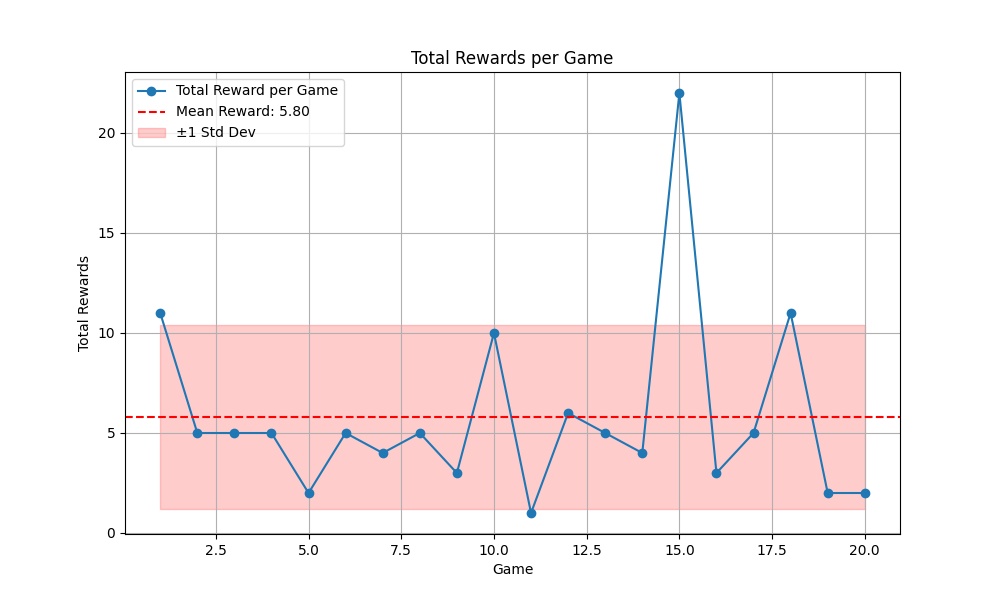
\includegraphics[width=0.8\textwidth]{rewards2.png}
%   \caption{Network Architecture}
%   \label{fig:network_architecture}
% \end{figure}

\subsection{Environment setup}
We use the KnightsArchersZombies environment from PettingZoo to train our model. The environment is initialized with
the following configuration:
\begin{itemize}
  \item Spawn Rate:15
  \item Number of Archers: 2
  \item Number of Knights: 2
  \item Maximum number of Zombies in an episode: 30
\end{itemize}

Before passing the state to the network, we preprocess the state using SuperSuit \cite{SuperSuit} wrappers by resizing it to 84 by 84 pixels and
converting it to grayscale.


\begin{table}[h]
  \caption{Hyperparameters}
   \centering
   \begin{tabular}{ll}
     \toprule
     hyperparameter     & value     \\
     \midrule
     total timesteps & $10000$ \\
     rollout size & $5000$ \\
     data buffer capacity & $8000$ \\
     reward scale & $1$ \\
     epochs & $6$ \\
     minibatch size & $256$ \\
     clip epsilon & $0.2$ \\
     value coefficient & $0.5$ \\
     entropy coefficient & $0.03$ \\
     discount factor & $0.99$ \\
     GAE lambda & $0.95$ \\
     value loss & $0.5$ \\
     huber delta & $10$ \\
     optimizer & Adam \\
     optimizer learning rate & $0.00005$ \\
     network initialization & Orthogonal \\
     \bottomrule
   \end{tabular}
   \label{tab:table}
 \end{table}


We train the model for 10,000 timesteps with a rollout size of 5000 and a data buffer capacity of 8000.


\subsection{Results}

\begin{figure}[h]
  \centering
  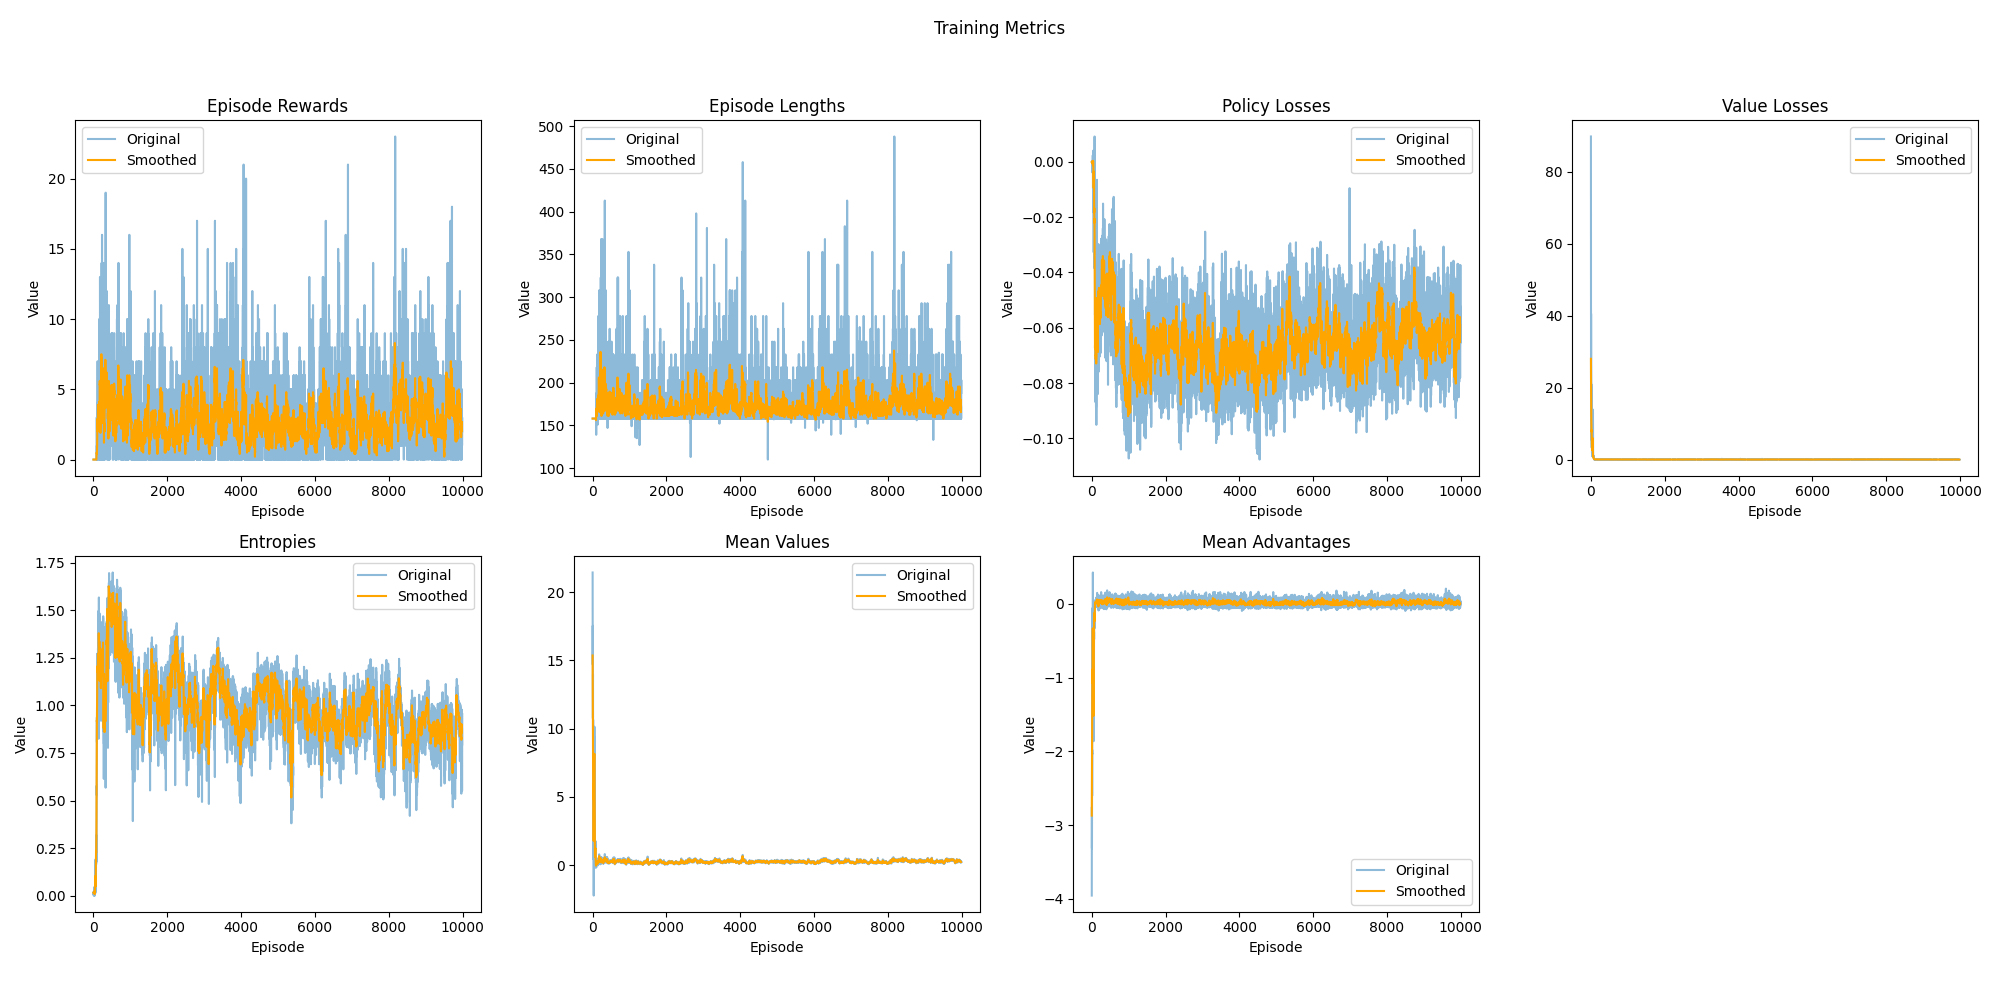
\includegraphics[scale=0.3]{run6.png}
  \caption{Training results}
  \label{fig:training_results_no_temporal}
\end{figure}

The training results show that the model converges to a suboptimal policy with a total reward of around 6 per episode. As the entropy 
of the policy decreases, it shows that exploration is decreasing and the policy is converging suboptimally. This suggests that the model is not learning
an effective strategy to kill the zombies. This could be due to the fact that the model is not able to capture zombie movement patterns properly. This makes it 
harder for the agent to predict zombies and targeting them effectively.

\section{Improved Implementation: Incorporating Temporal Data}
\subsection{Motivation for change}
The initial implementation did not perform well, suggesting that the model was not learning an effective policy. We hypothesized that the model
was not able to learn an effective policy because it was not able to capture the temporal dynamics of the environment properly. The model was only able to see
a single frame at a time, which made it hard capture patterns of movement and learn those details. 
To address this issue, we decided to incorporate temporal data into the model in the form of stacked frames.

\subsection{Changes to architecture}
We updated the network architecture to include a stack of 4 frames as input to the network. This allows the network to capture the temporal dynamics of the environment
and learn patterns of movement. The network architecture now consists of three convolutional layers followed by a fully connected layer. The input to the network is a stack of 4 frames
of size 84 by 84 pixels.

\subsection{Updates to environment setup}
We updated the environment setup to include a stack of 4 frames as input to the network. We used the SuperSuit wrappers to stack the frames before passing them to the network. We also modify
the entropy coefficient to a nonstandard value $0.04$ to encourage exploration and learning of a better policy.

\subsection{Results}
We see a drastic improvement in the performance of the model after incorporating temporal data. 
While not a lot, the total reward per episode has increased to around 10. The entropy of the policy is also higher, suggesting that the model is exploring more and learning a better policy.

\begin{figure}[h]
  \centering
  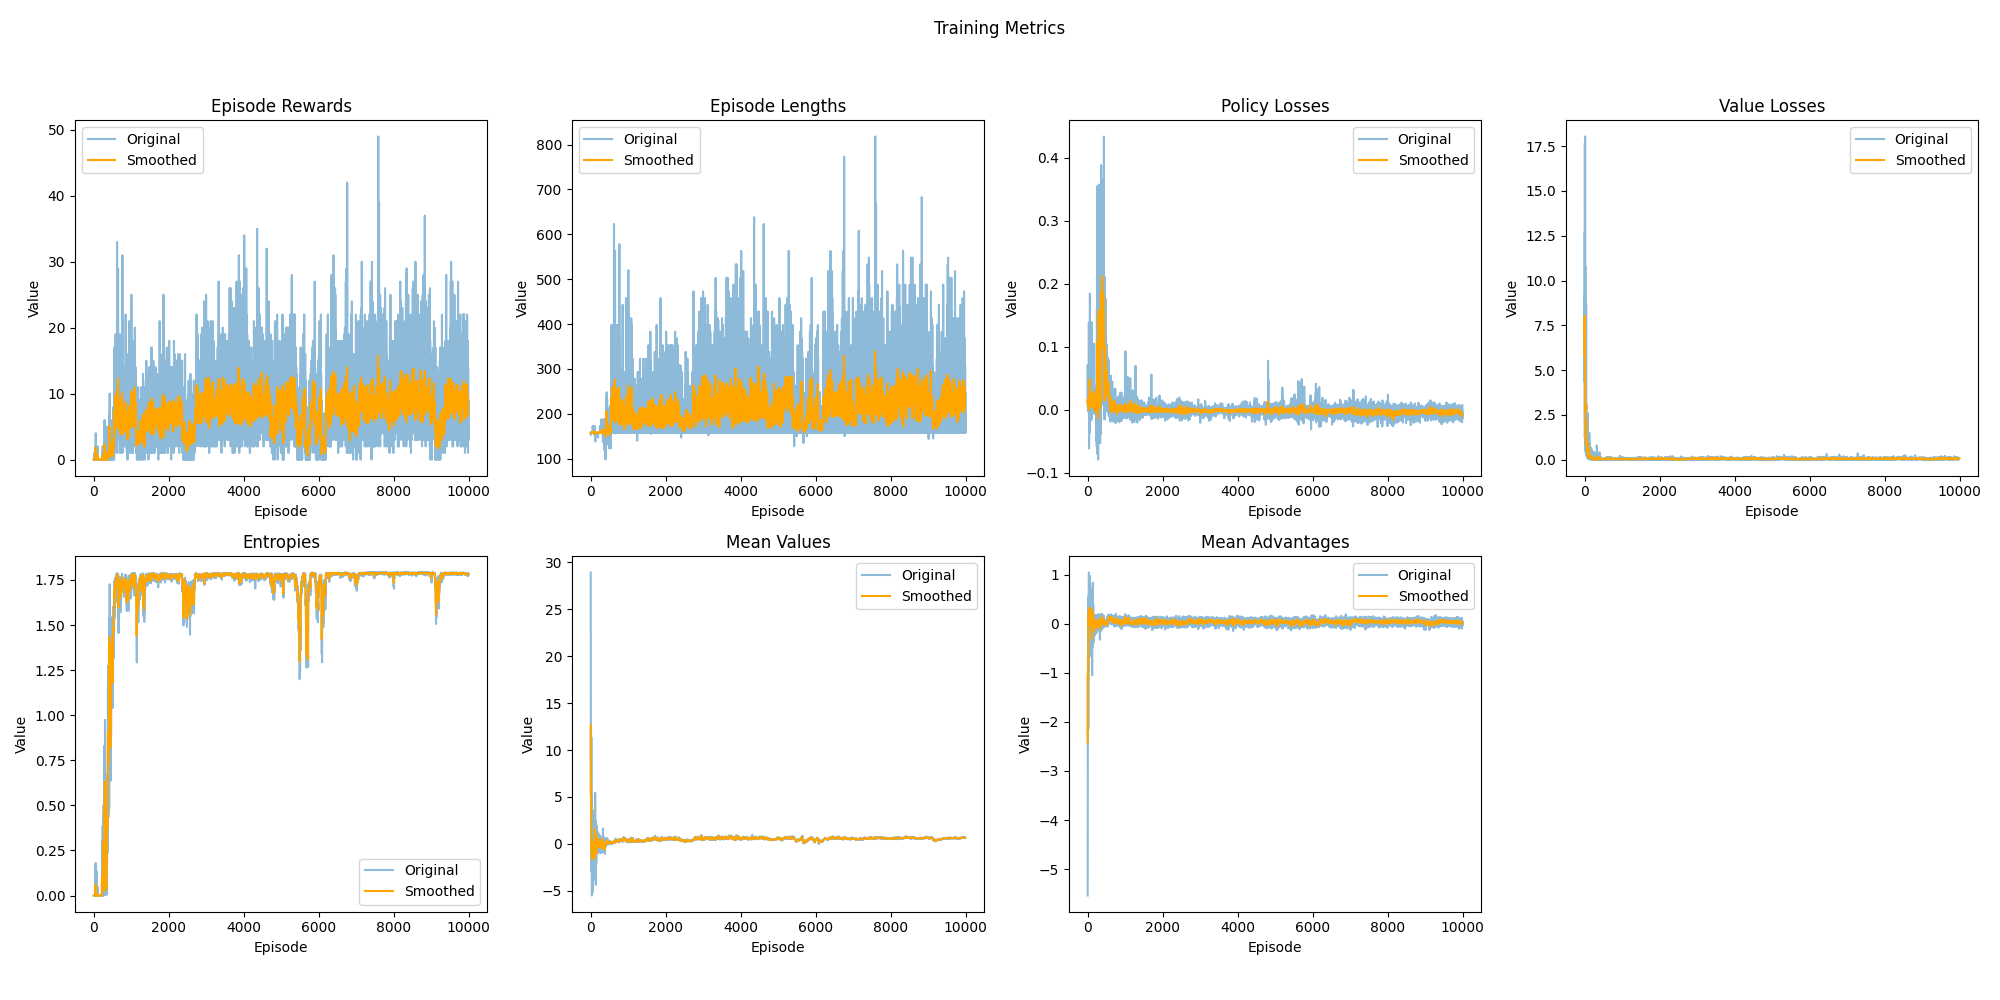
\includegraphics[scale=0.3]{run12.png}
  \caption{Training results with temporal data}
  \label{fig:training_results_with_temporal}
\end{figure}

The entropy of the policy is high till the very end, which means that it has kept exploring and learning throughout the training process. 
However, this also indicates that the model has not yet converged to an optimal policy and there is still room for improvement. We estimate that 
training for at least 50,000 timesteps would be required to reach a good policy. 


% \section{Observations}

\section{Emergent Behavior}
We find that the agents have learned to cooperate and target different directions, covering each other's blind spots and maximizing the number of zombies killed.
The agents have also learned to avoid the zombies and not collide with them, which is a good sign that the model is learning an effective policy.
Surprisingly, the agents have learned to predict zombies outside their observation limits (512 by 512 pixels) and move towards them, suggesting that the agents are learning to plan ahead and anticipate the movement of the zombies.


- Interesting observations\\
- Qualitative analysis of agent behavior\\
- Insights gained from the temporal data approach

\section{Discussion}

\subsection{Implications}
- Theoretical implications of the findings\\
  - hybrid centralized policy for all agents\\
- Why temporal data made a significant difference\\
- Broader insights into multi-agent reinforcement learning

\subsection{Limitations}
- Limitations of the current approach

\subsection{Future Work}
- Potential future work



\section{Conclusion}
Your conclusion here

\section*{Acknowledgments}
This was was supported in part by Professor Chris Amato and the CS 4180 course staff at Northeastern University.


%Bibliography
\bibliographystyle{unsrt}  
\bibliography{references}  

\end{document}

% \paragraph{Paragraph}
% \lipsum[7]

% \section{Examples of citations, figures, tables, references}
% \label{sec:others}
% \lipsum[8] \cite{DBLP:journals/corr/abs-2103-01955} and see \cite{DBLP:journals/corr/SchulmanWDRK17}.

% The documentation for \verb+natbib+ may be found at
% \begin{center}
%   \url{http://mirrors.ctan.org/macros/latex/contrib/natbib/natnotes.pdf}
% \end{center}
% Of note is the command \verb+\citet+, which produces citations
% appropriate for use in inline text.  For example,
% \begin{verbatim}
%    \citet{hasselmo} investigated\dots
% \end{verbatim}
% produces
% \begin{quote}
%   Hasselmo, et al.\ (1995) investigated\dots
% \end{quote}

% \begin{center}
%   \url{https://www.ctan.org/pkg/booktabs}
% \end{center}

% \subsection{Figures}
% \lipsum[10] 
% See Figure \ref{fig:fig1}. Here is how you add footnotes. \footnote{Sample of the first footnote.}
% \lipsum[11] 

% \begin{figure}
%   \centering
%   \fbox{\rule[-.5cm]{4cm}{4cm} \rule[-.5cm]{4cm}{0cm}}
%   \caption{Sample figure caption.}
%   \label{fig:fig1}
% \end{figure}

% \subsection{Tables}
% \lipsum[12]
% See awesome Table~\ref{tab:table}.

% \subsection{Lists}
% \begin{itemize}
% \item Lorem ipsum dolor sit amet
% \item consectetur adipiscing elit. 
% \item Aliquam dignissim blandit est, in dictum tortor gravida eget. In ac rutrum magna.
% \end{itemize}
